%%%%%%%%%%%%%%%%%%%%%%%%%%%%%%%%%%%%%%%%%%%%%%%%%%%%%%
% A Beamer template for University of Wollongong     %
% Based on THU beamer theme                          %
% Author: Qiuyu Lu                                   %
% Date: July 2024                                    %
% LPPL Licensed.                                     %
%%%%%%%%%%%%%%%%%%%%%%%%%%%%%%%%%%%%%%%%%%%%%%%%%%%%%%

\documentclass[serif, aspectratio=169]{beamer}
%\documentclass[serif]{beamer}  % for 4:3 ratio
\usepackage[T1]{fontenc} 
\usepackage{fourier} % see "http://faq.ktug.org/wiki/uploads/MathFonts.pdf" for other options
\usepackage{hyperref}
\usepackage{latexsym,amsmath,xcolor,multicol,booktabs,calligra}
\usepackage{graphicx,pstricks,listings,stackengine}
\usepackage{lipsum}
%\usepackage{subcaption}
%\usepackage[brazilian]{babel}
\usepackage{amsmath}
\usepackage{amsthm}
\usepackage{amssymb}
\usepackage{amsfonts}
\usepackage{graphicx}
\usepackage{physics}
\usepackage{csquotes}
\usepackage{geometry}
\usepackage{appendix}
\usepackage{indentfirst}
\usepackage{url}
\usepackage{hyperref}
\usepackage{subcaption}
\usepackage[super]{nth}
\usepackage{siunitx}
\graphicspath{ {images/} }
\newcommand{\ts}{\textsuperscript} %superscript
\newcommand{\av}[1]{\left\langle #1 \right\rangle} %prod int ou média
\newcommand{\R}{\mathbb{R}} %simbolo reais 
\newcommand{\tensor}{\overleftrightarrow} %seta dupla do tensor
\renewcommand{\curl}[1]{\nabla \times #1} %rotacional
\renewcommand{\div}[1]{\nabla \cdot #1} %divergente

%\newtheorem{theorem}{Teorema}[section]
%\newtheorem{example}{Exemplo}[section]

\usepackage[sorting=none, style=numeric]{biblatex}
\addbibresource{bibliography.bib}



\author{Arthur Diniz Meirelles \\
	\vspace{0.2cm}
	\small Advisor: Edivaldo Moura Santos \\
	\small Coadvisor: Ronaldo Carloto Batista}
\title{Optimization of the CMB-galaxy cross-correlation signal for studying the Integrated Sachs-Wolfe effect}
%\subtitle{Your Subtitle}
\institute{
    Institute of Physics \\
    Universidade de São Paulo
}
\date{\small 15/08/2024}
\usepackage{UoWstyle}

% defs
\def\cmd#1{\texttt{\color{red}\footnotesize $\backslash$#1}}
\def\env#1{\texttt{\color{blue}\footnotesize #1}}
\definecolor{deepblue}{rgb}{0,0,0.5}
\definecolor{deepred}{RGB}{153,0,0}
\definecolor{deepgreen}{rgb}{0,0.5,0}
\definecolor{halfgray}{gray}{0.55}

\lstset{
    basicstyle=\ttfamily\small,
    keywordstyle=\bfseries\color{deepblue},
    emphstyle=\ttfamily\color{deepred},    % Custom highlighting style
    stringstyle=\color{deepgreen},
    numbers=left,
    numberstyle=\small\color{halfgray},
    rulesepcolor=\color{red!20!green!20!blue!20},
    frame=shadowbox,
}


\begin{document}

\begin{frame}
	\titlepage
    \vspace*{-1.5cm}
    \begin{figure}[htpb]
    \centering
    \begin{subfigure}[t]{0.17\textwidth}
        \centering
        \includegraphics[width=\linewidth]{pic/USP-Brasão.jpg}
    \end{subfigure}
    %\hfill
    \begin{subfigure}[t]{0.25\textwidth}
        \centering
        \includegraphics[width=\linewidth]{pic/logo-ifusp-colorido_16.png}
    \end{subfigure}
    \hfill
    \begin{subfigure}[t]{0.25\textwidth}
        \centering
        \includegraphics[width=\linewidth]{pic/CNPq_logo.png}
    \end{subfigure}
    \end{figure}
\end{frame}

\begin{frame}    
\tableofcontents[sectionstyle=show,
subsectionstyle=show/shaded/hide,
subsubsectionstyle=show/shaded/hide]
\end{frame}

% Preamble and cover above

\section{Theoretical Aspects}

\begin{frame}{Introduction}
    \begin{columns}
        \column{0.5\linewidth}
        \begin{itemize}
        \item The integrated Sachs-Wolfe (ISW) effect occurs due to time changes in gravitational potentials;
        \item During periods of transition from or to matter-dominated eras of the Universe, potentials change more rapidly;
        \item Naturally, a statistical correlation between CMB temperature maps and gravitational potentials is expected.
        \end{itemize}
        \column{0.5\linewidth}
        \begin{figure}
            \centering
            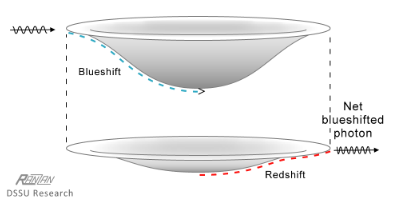
\includegraphics[width=\linewidth]{pic/ISW_illustration.png}
            \caption{Illustration of the ISW effect. In this case, the gravity wells flattened, leaving a net blueshift.}
            \label{fig:ISW_illustration}
        \end{figure}
    \end{columns}
\end{frame}

\begin{frame}{The $\Lambda$CDM Model}
    To build the theoretical framework used, it is assumed

    \begin{itemize}
        \item The Universe is homogeneous and isotropic at large scales; %talk about consequences
        \item Initial conditions are obtained by assuming an inflationary period when the Universe was very compact and energetic;
        \item The Universe is composed of baryonic matter, radiation, neutrinos, cold dark matter and a dark energy component described by a cosmological constant $\Lambda$;
    \end{itemize}

    The homogeneous and isotropic background is first set up, and linear perturbations are added to it.
\end{frame}

\begin{frame}{The Perturbed Metric}
	We express the perturbed metric with two functions $\Psi(\mathbf{x},t)$ and $\Phi(\mathbf{x},t)$
	
	\begin{equation}
	\begin{cases}
    		g_{00}=-1-2\Psi(\mathbf{x},t),\\
    		g_{0i}=g_{i0}=0,\\
    		g_{ij}=a^2(t)\delta_{ij}[1+2\Phi(\mathbf{x}, t)].
	\end{cases}
	\end{equation}
\end{frame}

%\begin{frame}{The $\Lambda$CDM Model}
%	The $\Lambda$CDM model explains some important observations, such as
%	
%	\begin{itemize}
%	\item The CMB and its properties;
%	\item The accelerating expansion of the Universe;
%	\item The Universe's large scale structure;
%	\end{itemize}
%	
%	And made some important predictions, like
%	
%	\begin{itemize}
%	\item Baryon accoustic oscillations (BAO);
%	\item The CMB polarization and its properties.
%	\end{itemize}
%\end{frame}

\begin{frame}{The $\Lambda$CDM Model}
	\begin{columns}
	
	\column{0.4\linewidth}
	\begin{figure}
	\centering
	\includegraphics[width=\linewidth]{pic/OmegaL_riess98.png}
	%\caption{Hubble diagram comparing different cosmological constants. Extracted from \cite{Riess_1998}.}
	%\label{fig:riess_OmegaL}
	\end{figure}
	
	\column{0.6\linewidth}
	\begin{figure}
	\centering
	\includegraphics[width=\linewidth]{pic/polarization_cross_spec.png}
	\end{figure}
	
	\end{columns}
\end{frame}

\begin{frame}{The Cosmic Microwave Background}
    The temperature of the Cosmic Microwave Background (CMB) can be expressed by

    \begin{equation}\label{eq:temp_def}
        T(\mathbf{x}, \hat{\mathbf{p}}, t)=\bar{T}(t)[1+\Theta(\mathbf{x}, \hat{\mathbf{p}}, t)].
    \end{equation}

    The temperature perturbation $\Theta$ can be expressed in Fourier space according to

    \begin{equation}\label{eq:Theta_expand}
        \Theta(\hat{\mathbf{k}}, \mu)=\sum_{\ell=0}^\infty (2\ell+1)(-i)^\ell \Theta_\ell(\hat{\mathbf{k}})\mathcal{P}_\ell(\mu),
    \end{equation}

    where $\mu=\hat{\mathbf{k}}\cdot \hat{\mathbf{p}}$ and $\mathcal{P}_\ell$ are Legendre polynomials.

    %\begin{align}
    %    \Theta_\ell&=\frac{1}{(-1)^\ell}\int_{-1}^1 \frac{\mathcal{P}_\ell(\mu) \Theta(\mu)}{2}d\mu, & \mu&=\hat{\mathbf{k}}\cdot \hat{\mathbf{p}}. 
    %\end{align}
\end{frame}

\begin{frame}{Analytical Approximation}
Working with first-order equations and the tightly coupled limit, and assuming recombination to be an instantaneous process happening at conformal time $\eta=\eta*$, we can obtain

\begin{equation}\label{Thetal_approx}
\begin{split}
    \Theta_\ell(k,\eta_0)\approx &[\Theta_0(k,\eta_*)+\Psi(k,\eta_*)]j_\ell[k(\eta_0-\eta_*)]\\
    &+iv_b(k,\eta_*)\left\{j_\ell[k(\eta_0-\eta_*)]-(\ell+1)\frac{j_\ell[k(\eta_0-\eta_*)]}{k(\eta_0-\eta_*)}\right\}\\
    &+\int_0^{\eta_0} d\eta e^{-\tau}[\Psi'(k,\eta)-\Phi'(k,\eta)]j_\ell[k(\eta_0-\eta)].
\end{split}
\end{equation}

Here, the third term in the equation describes the Integrated Sachs-Wolfe effect.
\end{frame}

\begin{frame}{Correlation Functions}
To calculate the CMB autocorrelation function $C_\ell^{tt}$, we expand $\Theta$ in spherical harmonics

\begin{equation}
    \Theta(\mathbf{x}, \hat{\mathbf{p}},t)=\sum_{\ell=1}^{\ell_\text{max}}\sum_{m=-\ell}^\ell a_{\ell m}(\mathbf{x},t)Y_{\ell m}(\hat{\mathbf{p}}),
\end{equation}

and calculate the autocorrelation between the $a_{\ell m}$ terms:

\begin{equation}
    \av{a_{\ell m} a_{\ell' m'}^*}=\delta_{\ell \ell'}\delta_{m m'}C_\ell^{tt}
\end{equation}

Other autocorrelation spectra $C_\ell^{xx}$ follow the same process. It is common to use $D_\ell^{XX}=\frac{\ell(\ell+1)}{2\pi}C_\ell^{xx}$ for some spectra for better visualization. We can also write

\begin{equation}
`	C_\ell^{tt}=\frac{1}{2\ell+1}\sum_{m=-\ell}^\ell a_{\ell m}a_{\ell' m'}^*
\end{equation}

\end{frame}

\begin{frame}{Cosmic Variance}
    The low number of $a_{\ell m}$ coefficients for lower multipoles $\ell$ leads to a high uncertainty in this region called cosmic variance

    \begin{equation}\label{cosmic_variance}
        \left(\frac{\Delta C_\ell^{XX}}{C_\ell^{XX}}\right)_{CV}=\sqrt{\frac{2}{2\ell+1}}
    \end{equation}
\end{frame}

\begin{frame}{Planck 2018}
    \begin{columns}
        \column{0.55\linewidth}
        \begin{figure}
            \centering
            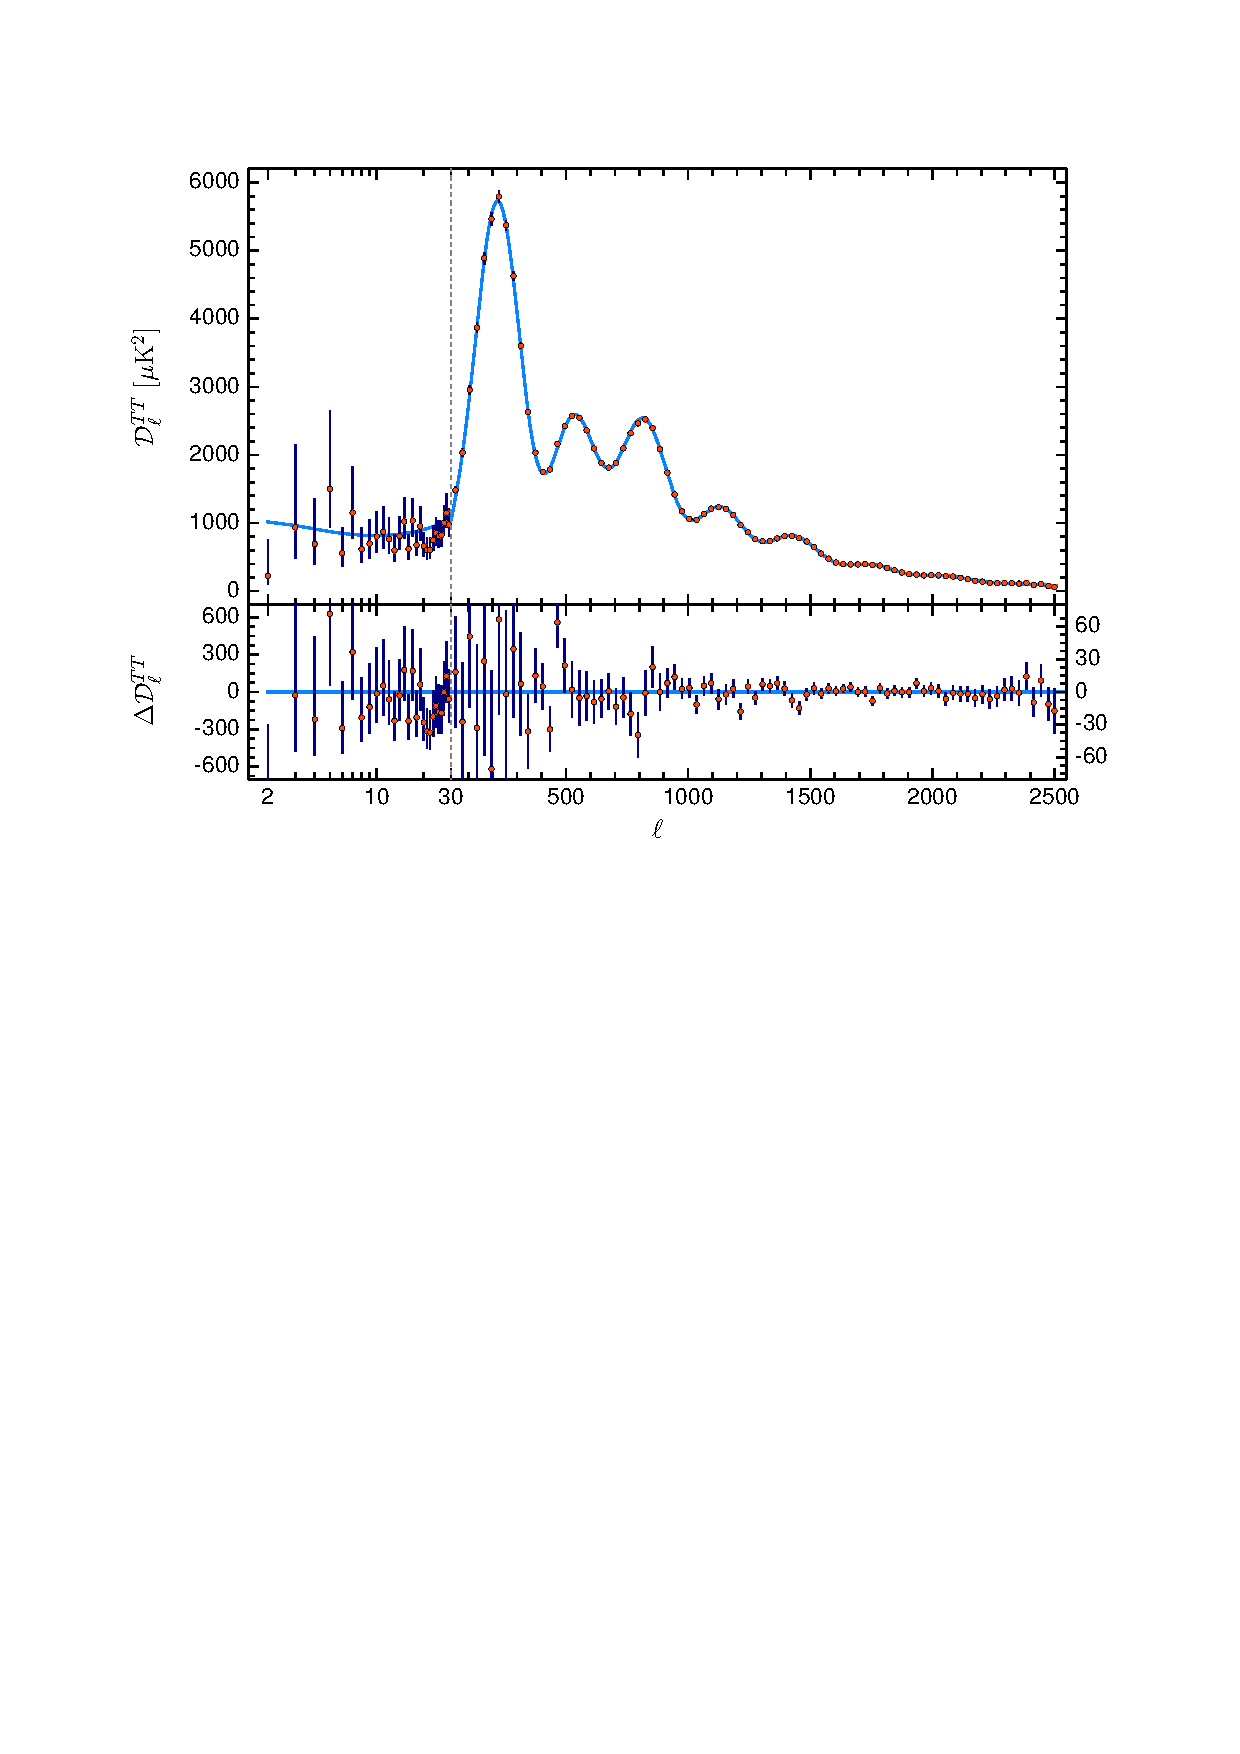
\includegraphics[width=\linewidth]{pic/planck_spectrum.pdf}
            \caption{Planck 2018 CMB temperature power spectrum.}
            \label{fig:planck_spectrum}
        \end{figure}
        \column{0.45\linewidth}
        \begin{table}[!htb]
    \centering
    \begin{tabular}{cc} \hline
     Parameter & Best-fit \\ \hline
     $\Omega_b h^2$ & $0.02237\pm 0.00015$\\
     $\Omega_c h^2$ & $0.1200\pm 0.0012$\\
     $100\Theta_{MC}$ & $1.04092\pm 0.00031$ \\
     $\tau$ & $0.0544\pm 0.0073$\\ 
     $\ln{(10^{10}A_s)}$ & $3.044 \pm 0.014$ \\ 
     $n_s$ & $0.9649 \pm 0.042$ \\ \hline
     %$\Omega_k$ & $0.0$ \\ \hline
     $\Omega_m$ & $0.3153 \pm 0.0073$ \\
     $H_0$ & $67.36 \pm 0.54$ km/s/Mpc \\
     $\sigma_8$ & $0.8111 \pm 0.0060$ \\ \hline
    \end{tabular}
    \caption{Best-fit values of cosmological parameters reported in Planck 2018 results using TT+TE+EE+lowE and gravitational lensing data.}
    \label{tab:planck_parameters}
\end{table}
    \end{columns}
\end{frame}

\begin{frame}{The Matter Power Spectrum}
    \begin{columns}
    \column{0.4\linewidth}
    	To calculate a cross-correlation function, we need the 3D matter power spectrum $P(k,z)$, defined by
    	
    \begin{equation*}
        \av{\delta(\mathbf{k},z) \delta^*(\mathbf{k}',z)}=(2\pi)^3 P(k,z)\delta_D(\mathbf{k}-\mathbf{k}')
    \end{equation*}
    
        We have used CAMB's implementation of the HALOFIT model to calculate the matter power spectrum.
        
    \column{0.6\linewidth}
    \begin{figure}
        \centering
        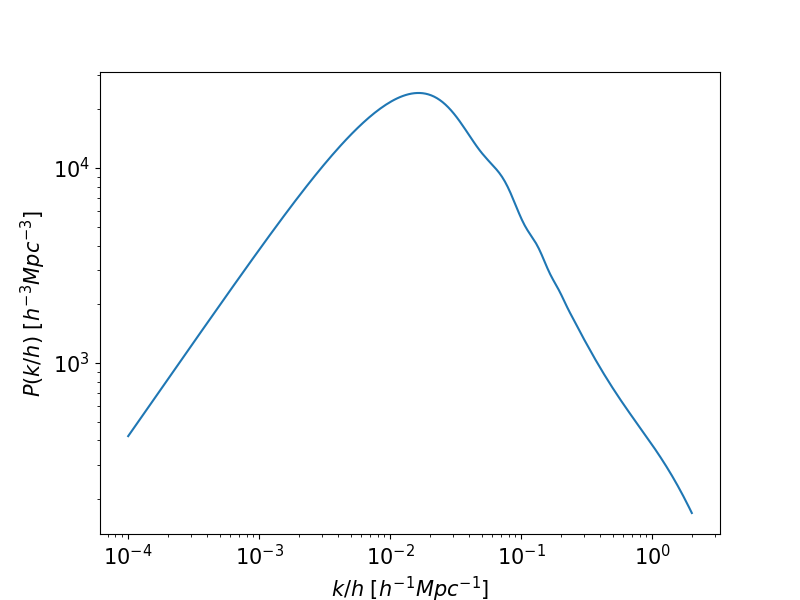
\includegraphics[width=0.9\linewidth]{pic/Pk_3dmatter_LCDM.png}
        \caption{Matter power spectrum calculated using both a linear approximation and the HALOFIT model.}
        \label{fig:Pk3dmatter}
    \end{figure}
\end{columns}
\end{frame}

\begin{frame}{The Cross-correlation Spectrum}
    To trace the matter density anisotropies, we used galaxy contrast maps, which can be calculated using

    \begin{equation}
        \delta_g(\mathbf{n})=\frac{N_g(\mathbf{n})-\bar{N}_g}{\bar{N}_g}
    \end{equation}

    It is assumed that $\delta_g=b_g\delta$, where $b_g$ is the bias factor, which we assume to be a slowly varying function of redshift. 

    The galaxy autocorrelation $C_{\ell}^{gg}$ and cross-correlation function $C_\ell^{tg}$ can then be calculated with

    \begin{align}
        \av{a_{\ell m}^t a_{\ell'm'}^g}&=C_\ell^{tg}\delta_{\ell \ell'}\delta_{mm'} & \av{a_{\ell m}^g a_{\ell'm'}^g}&=C_\ell^{gg}\delta_{\ell \ell'}\delta_{mm'}
    \end{align}
\end{frame}

\begin{frame}{Analytical Formula}
    Given fields x and y, representing either the ISW contribution to the CMB temperature ($x,y=t$) or the galaxy contrast ($x,y=g$), we can calculate the associated auto- or cross-correlation spectra using \cite{Moura-Santos_2016}

    \begin{equation}
        C_\ell^{xy}=\frac{2}{\pi}\int dk k^2 W_\ell^x(k)W_\ell^y(k)P(k),
    \end{equation}

    with

    \begin{equation}
        W_\ell^t=-3\Omega_m\left(\frac{H_0}{k}\right)^2\int dz \dv{[(1+z)D(z)]}{z}j_\ell[k\chi(z)]
    \end{equation}
    \begin{equation}\label{Wg}
        W_\ell^g=\int dz b_g(z)\dv{N}{z}D(z)j_\ell[k\chi(z)]
    \end{equation}
\end{frame}

\begin{frame}{ISW Contribution: Temperature Autocorrelation}
    \begin{figure}
        \centering
        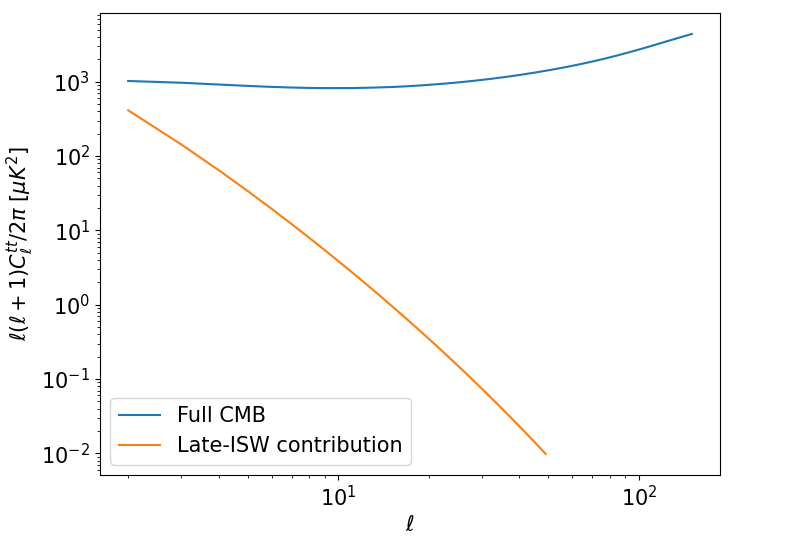
\includegraphics[width=0.65\linewidth]{pic/Ctt_comparison.png}
        \caption{CMB autocorrelation comparison between full spectrum and ISW contribution.}
        \label{fig:ISWplots_Ctt}
    \end{figure}
\end{frame}

\begin{frame}{ISW Contribution: Galaxy Autocorrelation and Cross-correlation}
    \begin{figure}
        \centering
        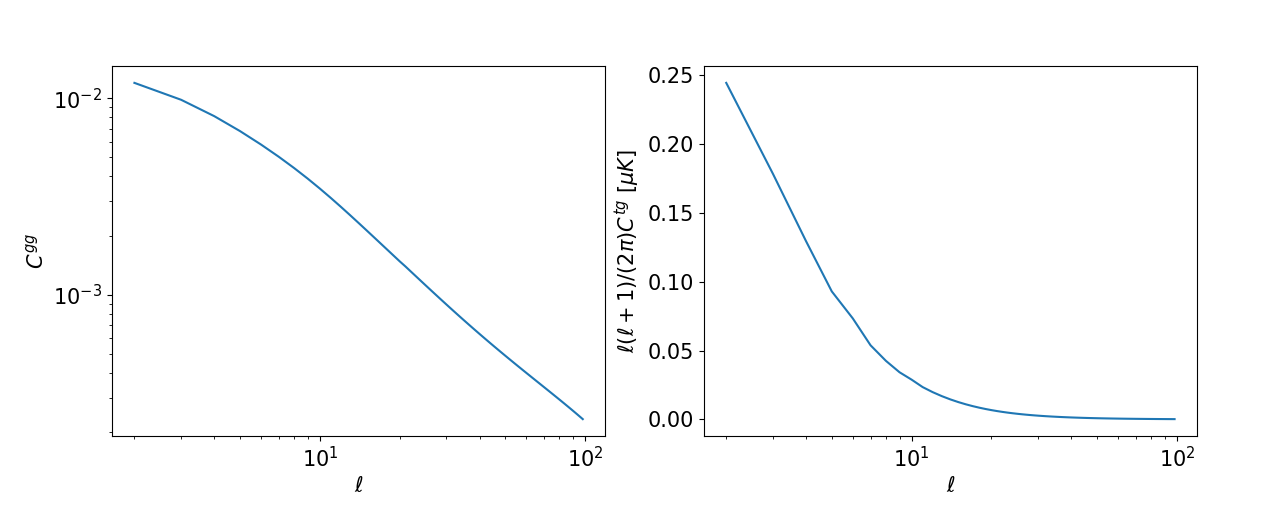
\includegraphics[width=\linewidth]{pic/Correlations_DoublePlot.png}
        \caption{Galaxy autocorrelation spectrum (left) and late-ISW contribution to the galaxy-CMB
cross-correlation (right).}
        \label{fig:ISWplots_Cgg_and_Ctg}
    \end{figure}
\end{frame}

\iffalse %Everything below this and before \fi is commented
%All frames commented will be highlighted
\begin{frame}{Dark Energy Models} %commented
	\begin{columns}
	\column{0.5\linewidth}
	
	Some alternative dark energy models allow for time varying equations of state. One of the most common parametrizations is the so called Chevallier-Polarski-Linder (CPL) parametrization:
	
	\begin{equation}
		w(z)=w_0+\left(1-\frac{1}{1+z}\right)w_a
	\end{equation}
	
	\column{0.5\linewidth}
	
	\begin{table}[!htb]
    \centering
    \begin{tabular}{cc} \hline
     Parameter & Marginalized Value \\ \hline
     $w_0$ & $-0.957\pm0.080$\\
     $w_a$ & $-0.29\substack{+0.32 \\ -0.26}$\\
     $H_0 [\text{km s}^{-1}\text{Mpc}^{-1}]$ & $68.31\pm0.82$ \\
     $\sigma_8$ & $0.820\pm 0.011$\\ \hline
     $\Delta \chi^2$ & -1.4 \\ \hline
    \end{tabular}
    \caption{Marginalized values and $68\%$ confidence limits for cosmological parameters, assuming the CPL parametrization.}
    \label{tab:planck_CPL}
\end{table}
	\end{columns}
\end{frame}

\begin{frame}{Dark Energy Models}%commented

    \begin{figure}
        \centering
        \begin{subfigure}[b]{0.32\linewidth}
            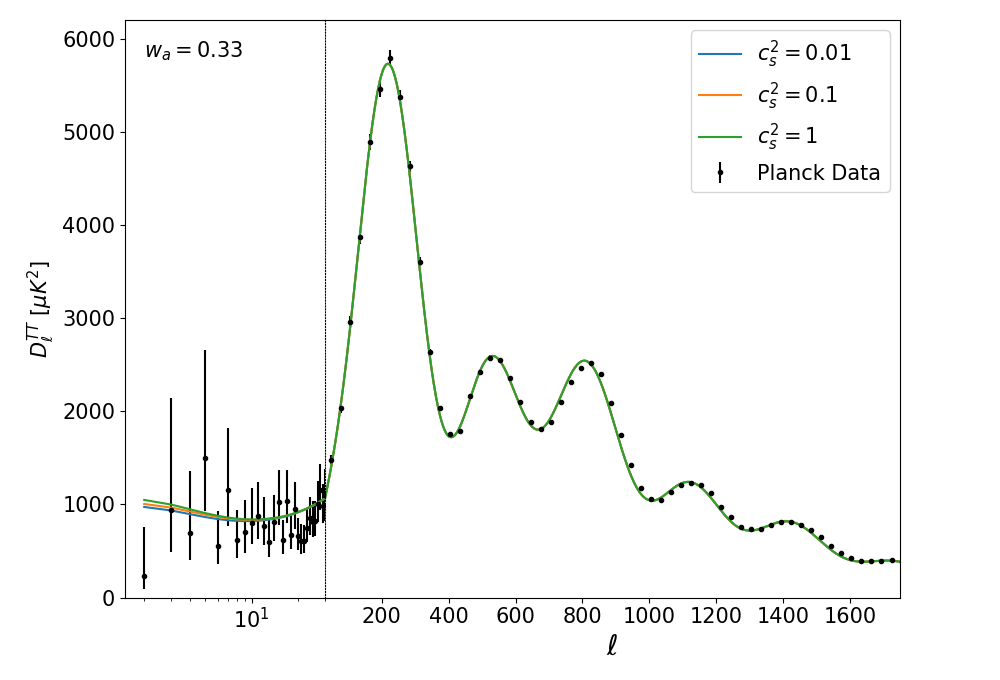
\includegraphics[width=\linewidth]{pic/full_doublscale_Wafixo0.33.png}
            %\caption{Cap 1}
            \label{fig:DE_wa033}
        \end{subfigure}
        \hfill
        \begin{subfigure}[b]{0.32\linewidth}
            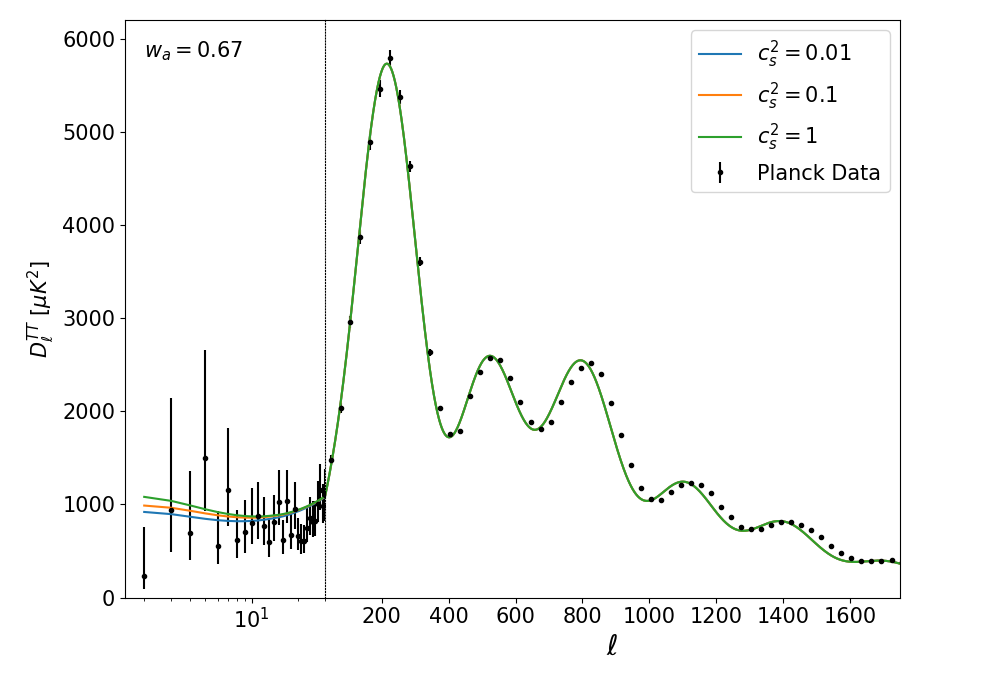
\includegraphics[width=\linewidth]{pic/full_doublscale_Wafixo0.67.png}
            %\caption{Cap 2}
            \label{fig:DE_wa067}
        \end{subfigure}
        \hfill
        \begin{subfigure}[b]{0.32\linewidth}
            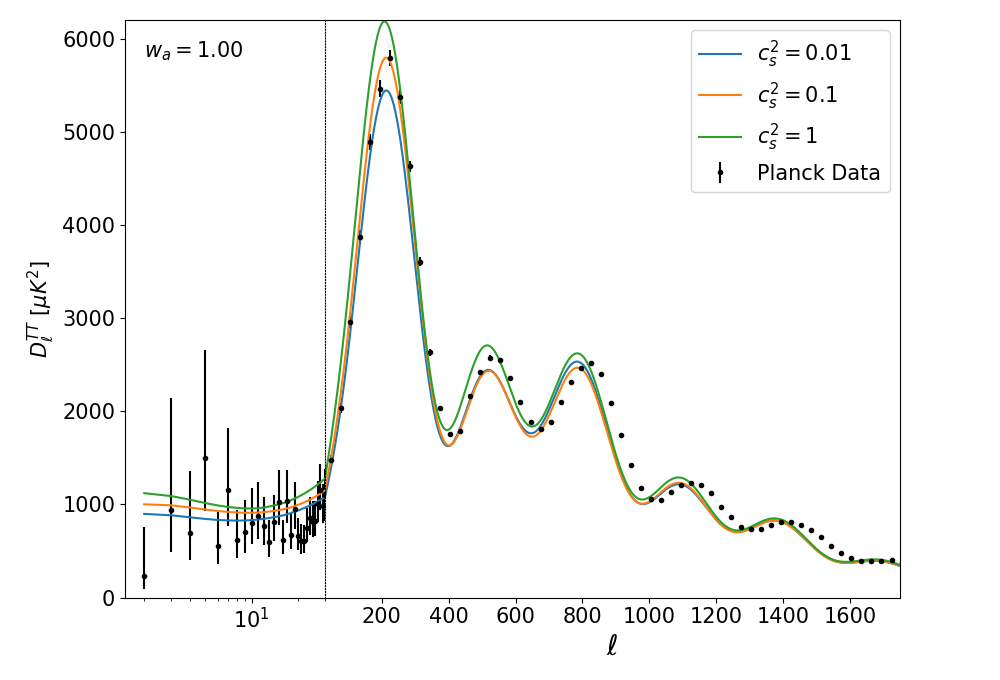
\includegraphics[width=\linewidth]{pic/full_doublscale_Wafixo1.00.png}
            %\caption{Cap 3}
            \label{fig:DE_wa1}
        \end{subfigure}
    \caption{CMB temperature autocorrelation spectrum calculated with parameter combinations using the CPL parametrization.}
    \label{fig:DE_wa_fixo}
    \end{figure}

\end{frame}

\begin{frame}{Dark Energy Models}%Commented

    \begin{figure}
        \centering
        \begin{subfigure}[b]{0.32\linewidth}
            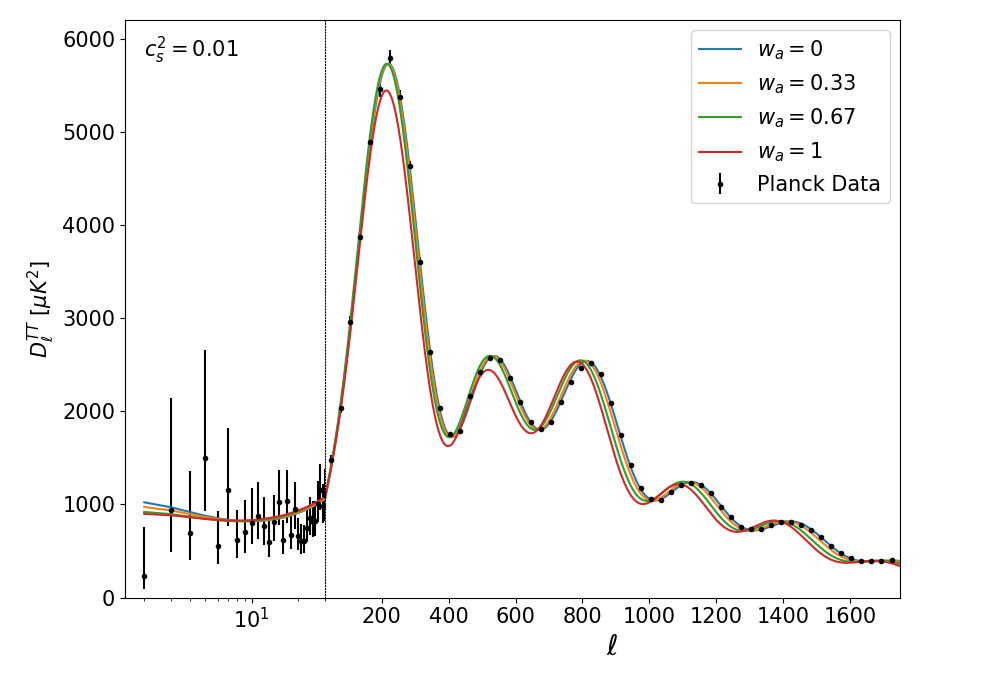
\includegraphics[width=\linewidth]{pic/full_doublscale_Cs2fixo0.01.png}
            %\caption{Cap 1}
            \label{fig:DE_cs001}
        \end{subfigure}
        \hfill
        \begin{subfigure}[b]{0.32\linewidth}
            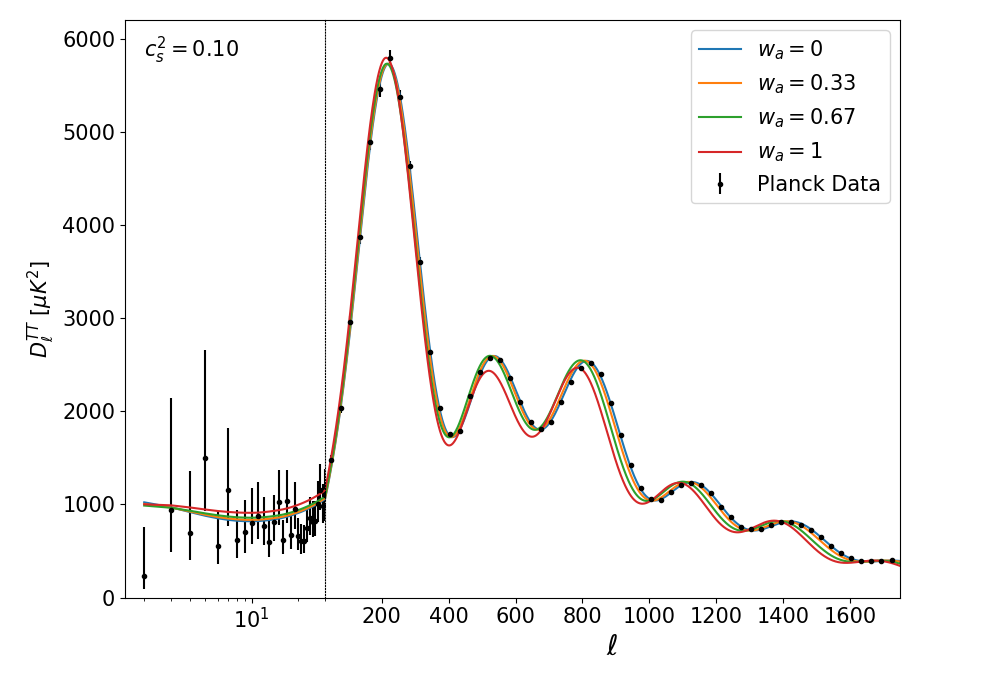
\includegraphics[width=\linewidth]{pic/full_doublscale_Cs2fixo0.10.png}
            %\caption{Cap 2}
            \label{fig:DE_cs01}
        \end{subfigure}
        \hfill
        \begin{subfigure}[b]{0.32\linewidth}
            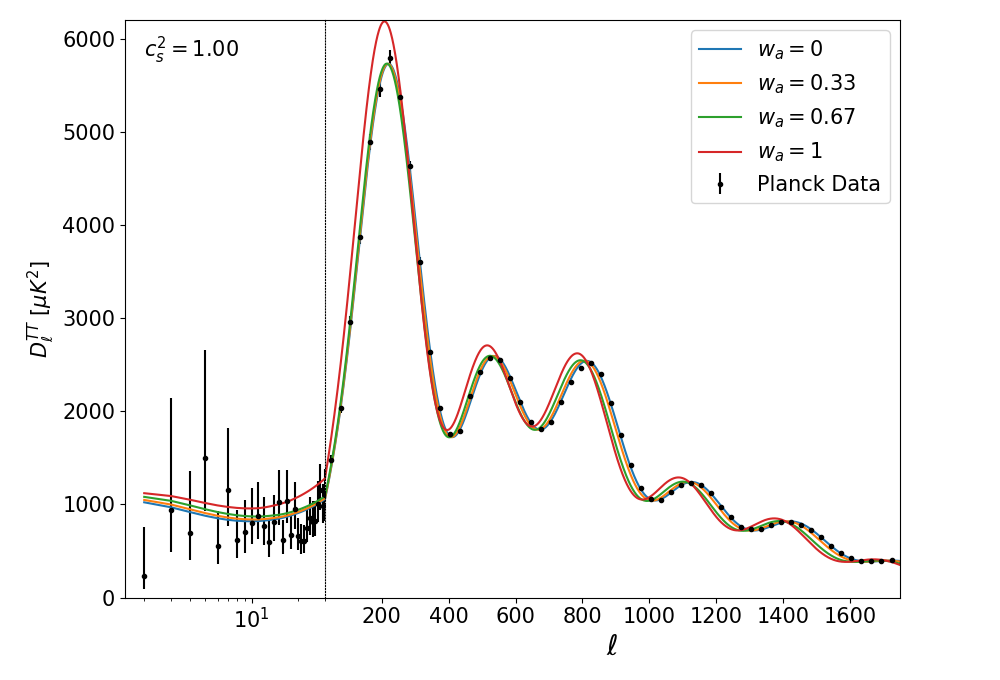
\includegraphics[width=\linewidth]{pic/full_doublscale_Cs2fixo1.00.png}
            %\caption{Cap 3}
            \label{fig:DE_cs1}
        \end{subfigure}
    \caption{CMB temperature autocorrelation spectrum calculated with parameter combinations using the CPL parametrization.}
    \label{fig:DE_cs_fixo}
    \end{figure}

\end{frame}
\fi

\section{Optimized Galaxy Survey}

\begin{frame}{Selection Function Parametrization}
    The function $\dv{N}{z}$ in equation \eqref{Wg} is called the selection function. We are assuming its parametrization to be \cite{select_func_par:Afshordi2004}

    \begin{equation}\label{select_func_par}
        \dv{N}{z}\left(z|\lambda, \beta, z_0\right)dz=\frac{\beta}{\Gamma(\lambda)}\left(\frac{z}{z_0}\right)^{\beta\lambda-1}\text{exp}\left[-\left(\frac{z}{z_0}\right)^\beta\right]d\left(\frac{z}{z_0}\right)
    \end{equation}

    We have explored how to maximize the cross-correlation signal using an idealized selection function.
\end{frame}

\begin{frame}{2MASS Bands Comparison}
    \begin{columns}
        \column{0.55\linewidth}
        \begin{figure}
            \centering
            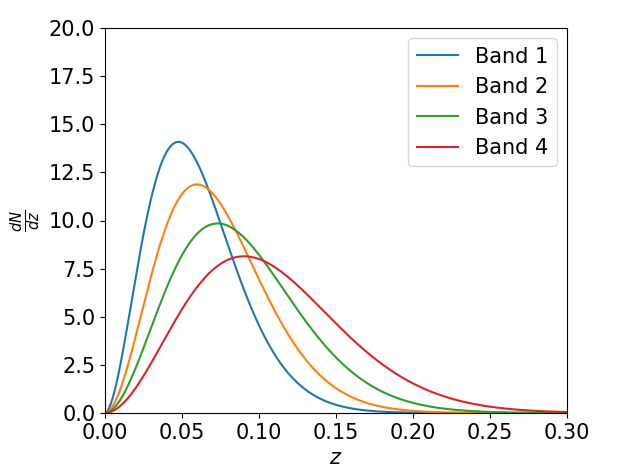
\includegraphics[width=\linewidth]{pic/selection_2MASS.png}
            \caption{Selection function calculated for the 4 bands of the 2MASS catalog.}
            \label{fig:selection_2MASS}
        \end{figure}
    
        \column{0.45\linewidth}
        \begin{table}[!htb]
            \centering
            \begin{tabular}{cccc} \hline
             Band & $z_0$ & $\beta$ & $\lambda$ \\ \hline
             1 & $0.043$ & $1.825$ & $1.524$\\
             2 & $0.054$ & $1.800$ & $1.600$ \\
             3 & $0.067$ & $1.765$ & $1.636$\\
             4 & $0.084$ & $1.723$ & $1.684$\\ \hline
            \end{tabular}
            \caption{Parameter values for the 4 bands of the 2MASS catalog.}
            \label{tab:bands_2MASS}
        \end{table}
    \end{columns}
\end{frame}

\begin{frame}{Exploring the Parameter Space}
    \begin{figure}
        \centering
        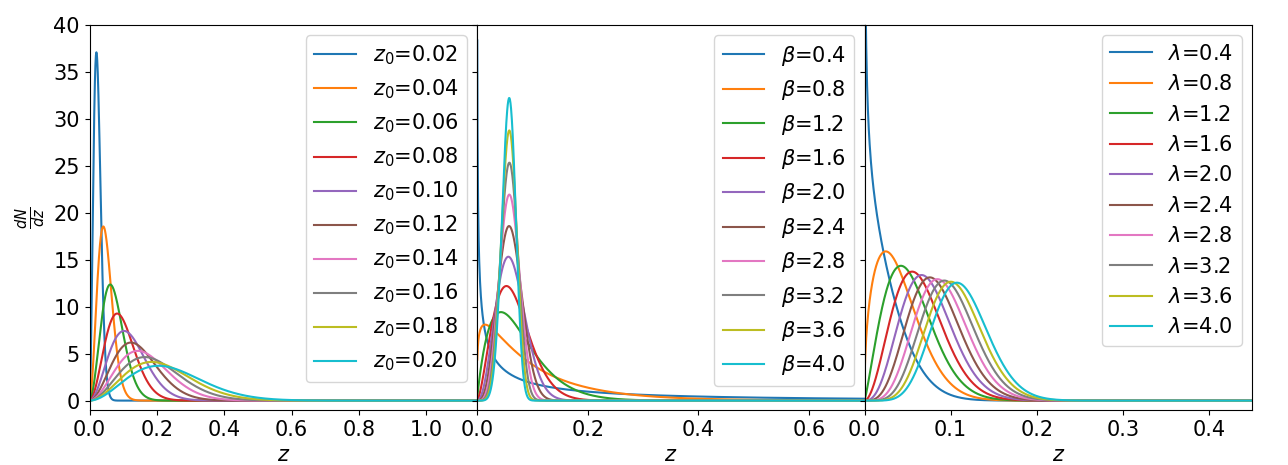
\includegraphics[width=\linewidth]{pic/Selection_TriplePlot.png}
        \caption{Selection function calculated for various parameter values.}
        \label{fig:selection_triplePlot}
    \end{figure}
\end{frame}

\begin{frame}{Null Hypothesis}
    For the process of finding a galaxy survey with an idealized selection function, we first needed an estimation for the probability of $C_\ell^{tg}$ being 0, which would be our null hypothesis. The following process was used: 

    \begin{itemize}
        \item Synthesize multiple uncorrelated CMB temperature and galaxy contrast maps using HEALPix;
        \item Calculate the cross-correlation $C_\ell^{tg}$ for each pair of uncorrelated maps at each multipole;
        \item For each multipole $\ell$, a histogram of $C_\ell^{tg}$ was produced;
        \item Each histogram was fit with Gaussian distributions with average $\mu=\mu_\ell\approx 0$ and $\sigma^2=\sigma_\ell^2$.
    \end{itemize}
    
    The null hypothesis is compatible with $\Omega_m=1$.
\end{frame}

\begin{frame}{Synthesized Maps' Histograms}
    \begin{figure}

        \begin{subfigure}[b]{0.45\linewidth}
            \centering
            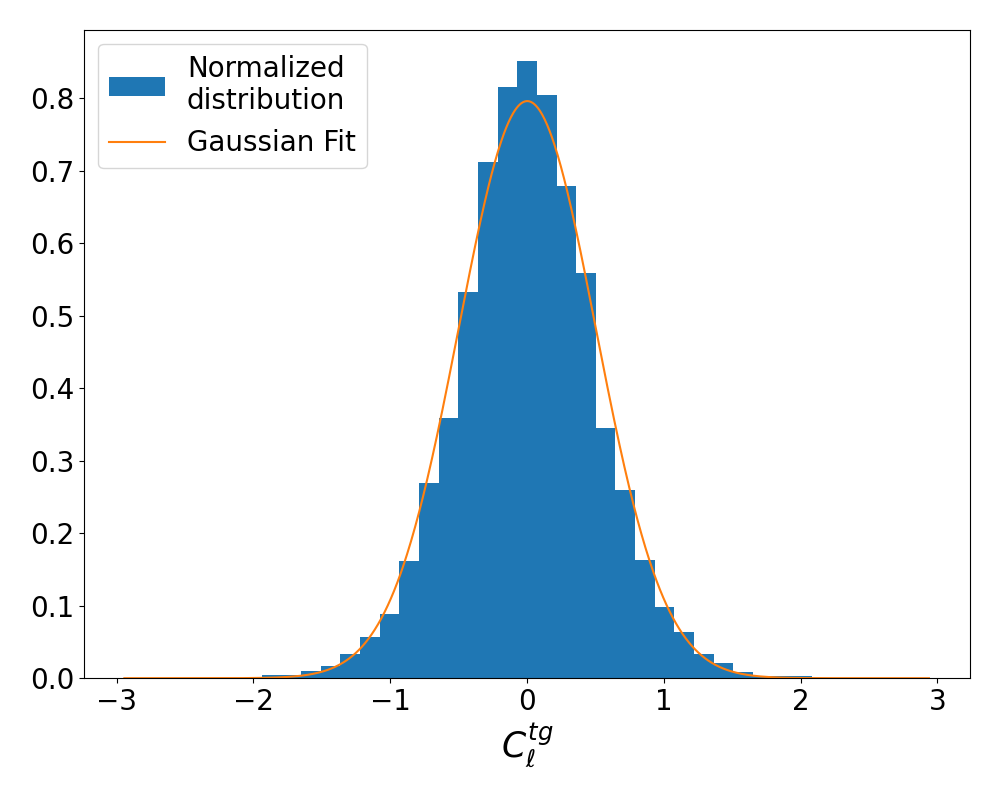
\includegraphics[width=\linewidth]{pic/hist_l4.png}
            \caption{$\ell=4$}
            \label{fig:hist_l4}
        \end{subfigure}
        \hfill
        \begin{subfigure}[b]{0.45\linewidth}
            \centering
            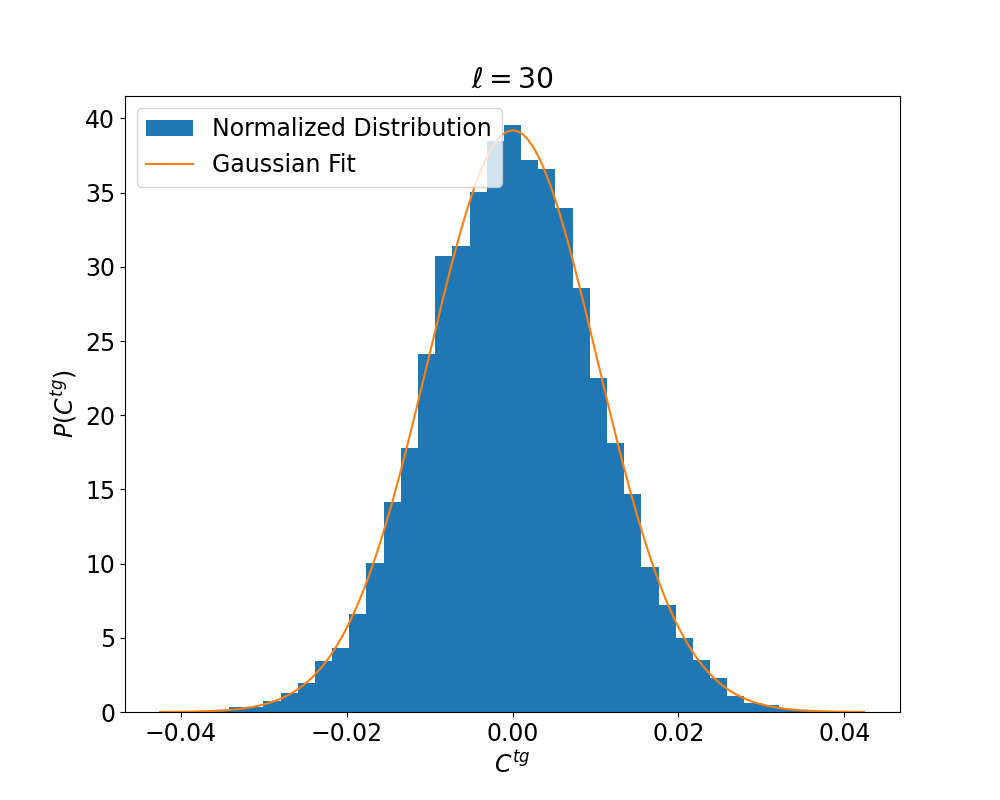
\includegraphics[width=\linewidth]{pic/hist_l30.png}
            \caption{$\ell=30$}
            \label{fig:hist_l30}
        \end{subfigure}
        
        \caption{Distribution of cross-correlation values on different multipoles for $10^4$ maps synthe-
sized with null cross-correlation.}
        \label{fig:hists}
    \end{figure}
\end{frame}

\begin{frame}{Null Hypothesis}
    For $f_\ell$ corresponding to the Gaussian fit made for the multipole $\ell$

    \begin{equation}
        f_\ell(C_\ell^{tg})=\frac{1}{\sqrt{2\pi \sigma_\ell^2}}\text{exp}\left[-\frac{1}{2}\left(\frac{C_\ell^{tg}-\mu_\ell}{\sigma_\ell}\right)^2\right],
    \end{equation}

    we have defined the null hypothesis probability distribution to be

    \begin{equation}
        P_\text{null}=\prod_{\ell=2}^{\ell_\text{max}} f_\ell(C_\ell^{tg})
    \end{equation}
\end{frame}

\begin{frame}{Exploring the Parameter Space}
    \begin{columns}
    \column{0.4\linewidth}
        For various points $(\beta, z_0, \lambda)$ in the parameter space, we have calculated the ratio $P_\text{null}(\beta, z_0, \lambda)/P_\text{null}^\text{2MASS}$ and produced the heat maps in Figure \ref{fig:HeatMaps}. 

    \column{0.6\linewidth}
    \begin{figure}
        \centering
        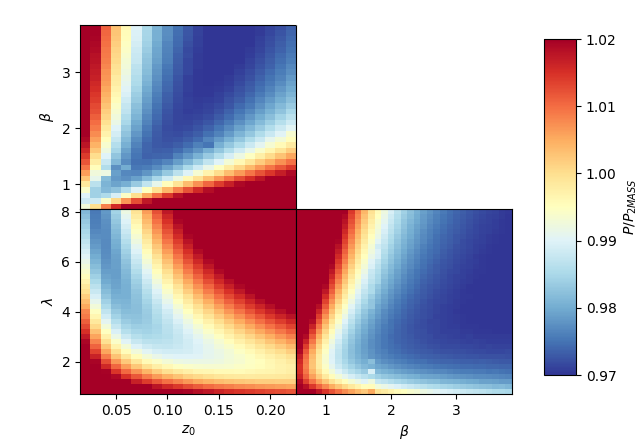
\includegraphics[width=\linewidth]{pic/triple_colorplot.png}
        \caption{Heat maps used to explore the parameter space.}
        \label{fig:HeatMaps}
    \end{figure}
    \end{columns}
\end{frame}

\begin{frame}{Minimizer}
    The heat maps provided initial points to run an algorithm that minimizes $P_\text{null}(z_0,\beta, \lambda)$. The point found that minimizes the null hypothesis probability in that region of the parameter space was

    \begin{equation}
        (\beta, z_0, \lambda)=(3.088, 0.1508, 4.9401)
    \end{equation}
\end{frame}

\begin{frame}{Properties of the Minimum}
\begin{columns}
    \column{0.6\linewidth}
    \begin{figure}
        \centering
        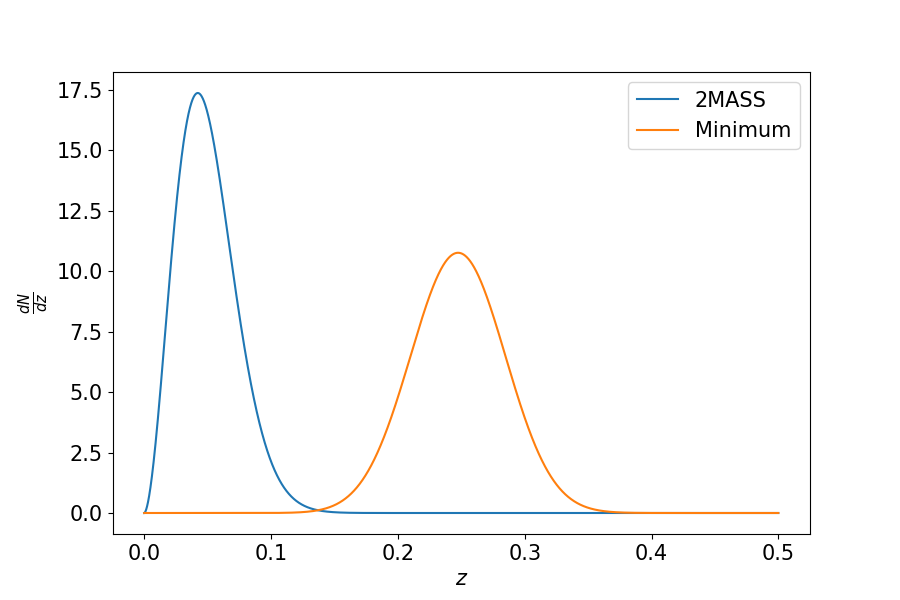
\includegraphics[width=\linewidth]{pic/minimum_SelFunc.png}
        \caption{Selection functions comparison.}
        \label{fig:minimum_SelFunc}
    \end{figure}
    \column{0.4\linewidth}
    The selection function found is deeper than that of 2MASS band 1. It does not favor galaxies at $z^*=0.63$, the estimated redshift at which the accelerated expansion started.
\end{columns}
\end{frame}

\begin{frame}{Properties of the Minimum}
    \begin{columns}
        \column{0.4\linewidth}
        The selection function found reduces the maximum value of the cross-correlation function, but its peak is at higher redshifts ($\ell\approx 10$), reducing the influence of cosmic variance in the signal.
        
        \column{0.6\linewidth}
        \begin{figure}
            \centering
            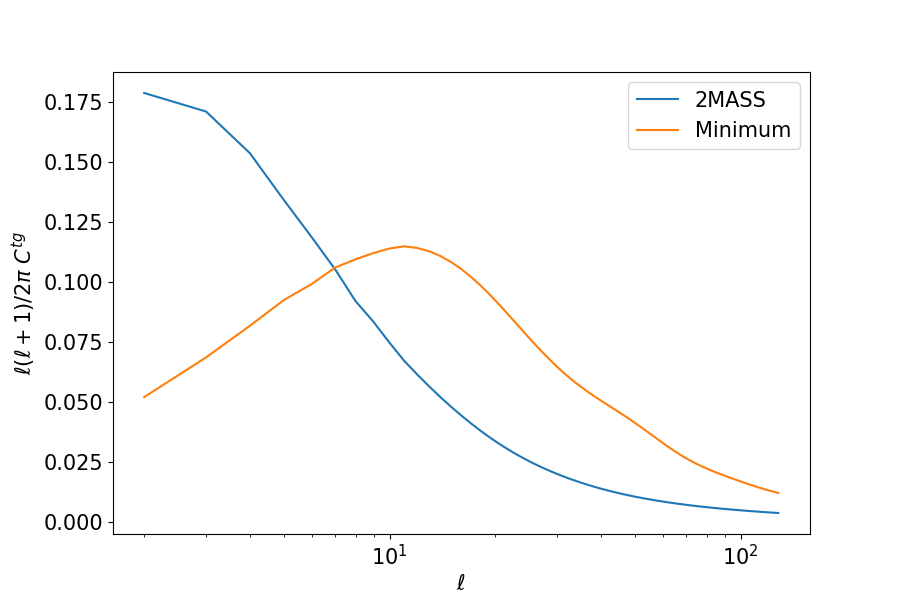
\includegraphics[width=\linewidth]{pic/minimumX2mass.png}
            \caption{Theoretical cross-correlation spectrum comparison.}
            \label{fig:minimum_cross_corr}
        \end{figure}
    \end{columns}
\end{frame}

\begin{frame}{Discussion}
    \begin{itemize}
        \item The ratio $P_\text{null}(z_0,\beta, \lambda)/P_\text{null}^\text{2MASS}=0.971$ for the minimum;
        \item Despite the small statistical gain, this optimal selection function yields reasonably better results for constraints on $\Omega_m$, as will be discussed;
        \item A similar work has reported a small preference towards the non-null signal with changes to the depth of the survey and fainter magnitude limits \cite{simillar_ISW_analysis}.
    \end{itemize}
\end{frame}

\section{Data Processing}

\begin{frame}{WMAP Data}
The CMB temperature maps used in this project are the ones provided by WMAP9 \cite{wmap_supplement}.

\begin{itemize}
	\item Three frequency bands were used, which are named bands Q ($40\text{GHz}$), V ($60\text{GHz}$) and W ($90\text{GHz}$);
	\item The temperature intensity maps' noise power can be well modeled as uncorrelated Gaussian fluctuations;
	\item Despite having a lower resolution ($0.3\degree$) compared to Planck's ($0.083\degree$), this project focuses on lower multipoles;
	\item We have combined both maps' masks and used it for analysing each one, resulting in a fraction $f_\text{sky}=0.7$.
\end{itemize}
\end{frame}

\begin{frame}{WMAP Data}
    \begin{figure}
        \centering
        \begin{subfigure}[b]{0.32\linewidth}
            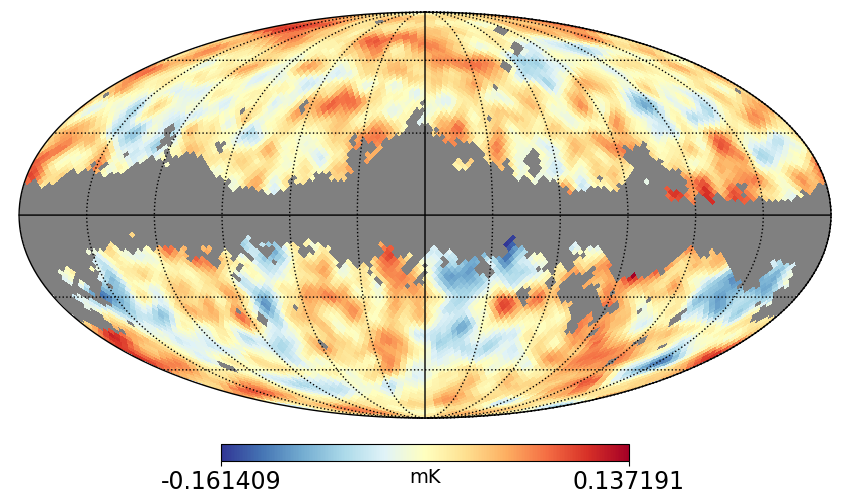
\includegraphics[width=\linewidth]{pic/wmap_Q_wmask.png}
            \caption{Q channel}
            \label{fig:wmap_Q}
        \end{subfigure}
        \hfill
        \begin{subfigure}[b]{0.32\linewidth}
            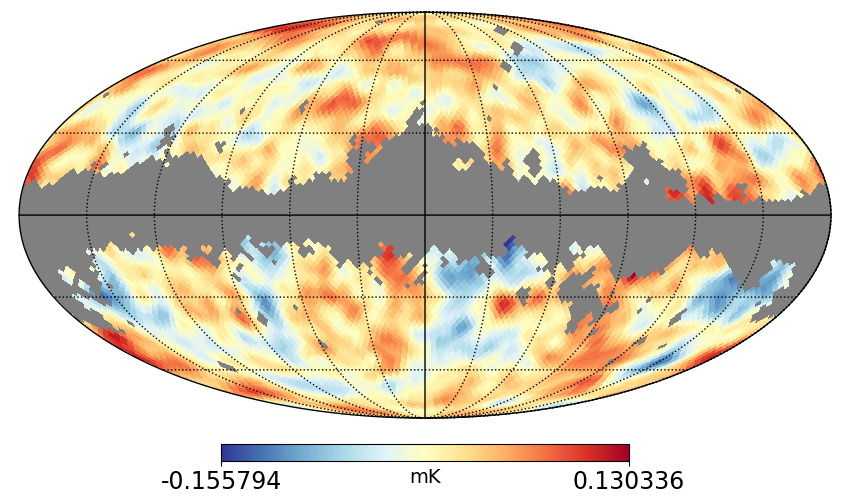
\includegraphics[width=\linewidth]{pic/wmap_V_wmask.png}
            \caption{V channel}
            \label{fig:wmap_V}
        \end{subfigure}
        \hfill
        \begin{subfigure}[b]{0.32\linewidth}
            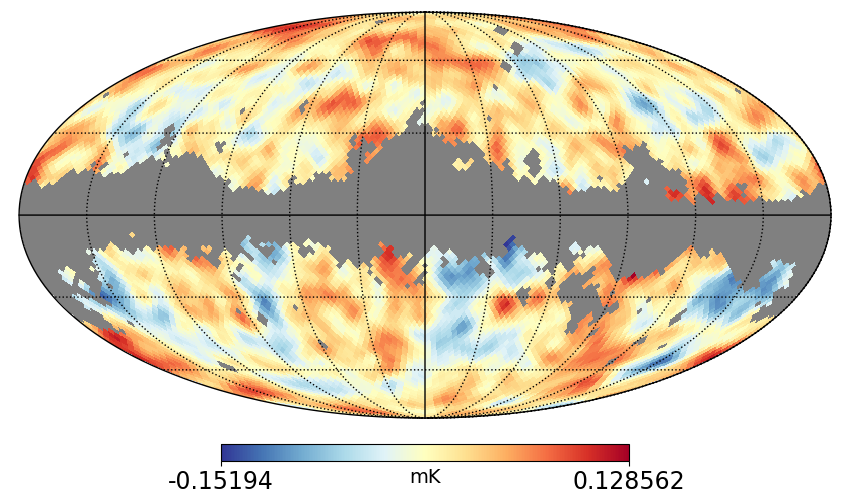
\includegraphics[width=\linewidth]{pic/wmap_W_wmask.png}
            \caption{W channel}
            \label{fig:wmap_W}
        \end{subfigure}
    \caption{Mollweide projection of three (Q, V, W) WMAP9 CMB temperature (in mK) maps in galactic coordinates with an $f_\text{sky}=0.70$ mask applied}
    \label{fig:wmap_maps}
    \end{figure}
\end{frame}

\begin{frame}{2MASS Catalog}
Wide sky coverage is a very influential aspect of studying cross-correlation spectra, and the 2MASS catalog contains raw imaging data covering $99.998\%$ of the sky \cite{2MASS}, which was the dataset used. 

\begin{itemize}
	\item We have used the $K_s$ ($\SI{2.16}{\mu \meter}$) band of the Extended Source Catalog (XSC);
	\item The data of the $K_s$ band obtained from a 20 mag aperture ($K_{20}$) were corrected for galactic extinction, and the remaining data was further divided into 4 bands: Bands 1 ($12.0<K_{20}'<12.5$), 2 ($12.5<K_{20}'<13.0$), 3 ($13.0<K_{20}'<13.5$) and 4 ($13.5<K_{20}'<14.0$);
	\item Each band has a different selection function, as shown in Figure \ref{fig:selection_2MASS}.
\end{itemize}
\end{frame}

\begin{frame}{2MASS Catalog}
    \begin{figure}
     \centering
     \begin{subfigure}[t]{0.49\textwidth}
         \centering
         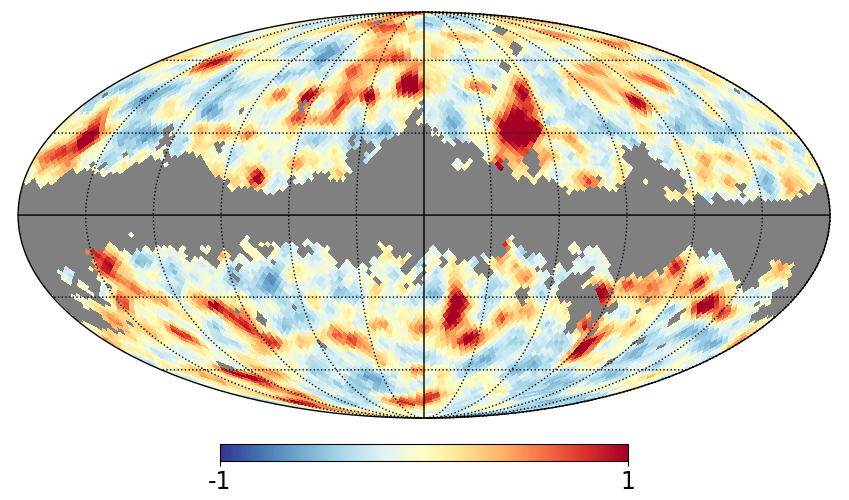
\includegraphics[width=\textwidth]{pic/band1_wmask_xsc.png}
         \caption{Band 1}
         \label{fig:contrast_map1}
     \end{subfigure}
     \hfill
     \begin{subfigure}[t]{0.49\textwidth}
         \centering
         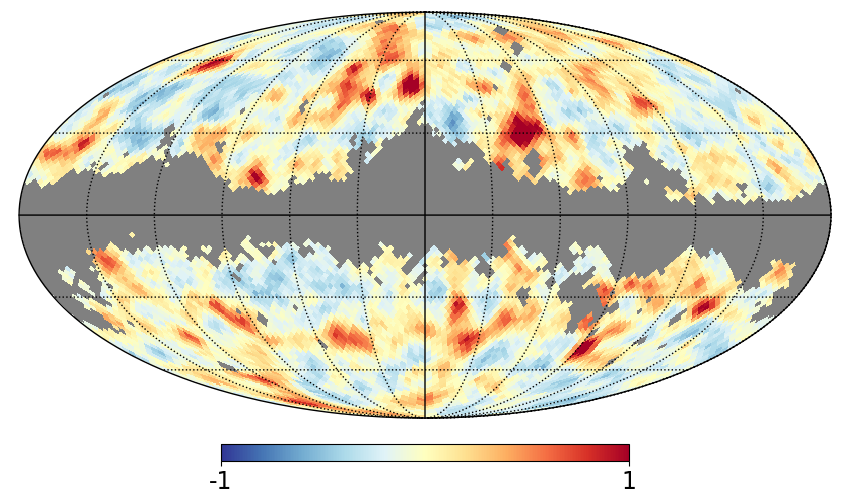
\includegraphics[width=\textwidth]{pic/band2_wmask_xsc.png}
         \caption{Band 2}
         \label{fig:contrast_map2}
     \end{subfigure}
     \caption{Mollweide projection of the 2MASS-XSC galaxy contrast maps in galactic coordinates with the combined 2MASS+WMAP mask applied ($f_{sky}=0.70$).}
        \label{fig:2MASS_maps1}
      \end{figure}
\end{frame}

\begin{frame}{2MASS Catalog}
    \begin{figure}
    \centering
        \begin{subfigure}[b]{0.49\textwidth}
             \centering
             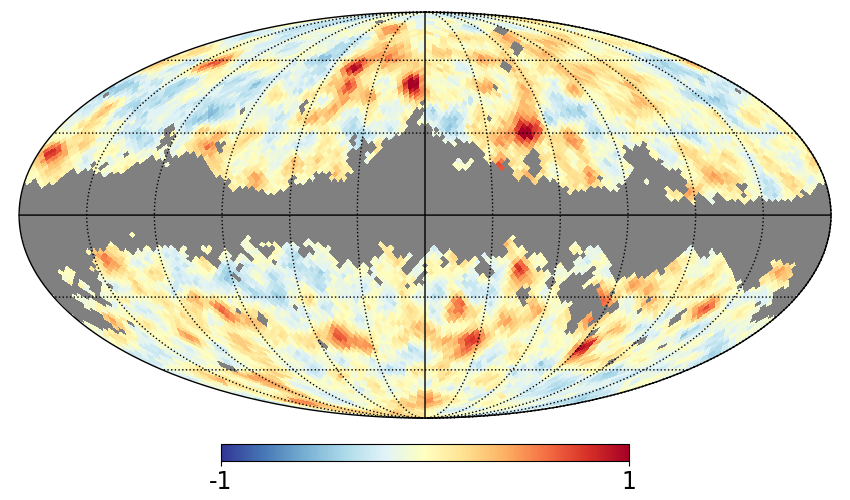
\includegraphics[width=\textwidth]{pic/band3_wmask_xsc.png}
             \caption{Band 3}
             \label{fig:contrast_map3}
        \end{subfigure}
        \hfill
        \begin{subfigure}[b]{0.49\textwidth}
             \centering
             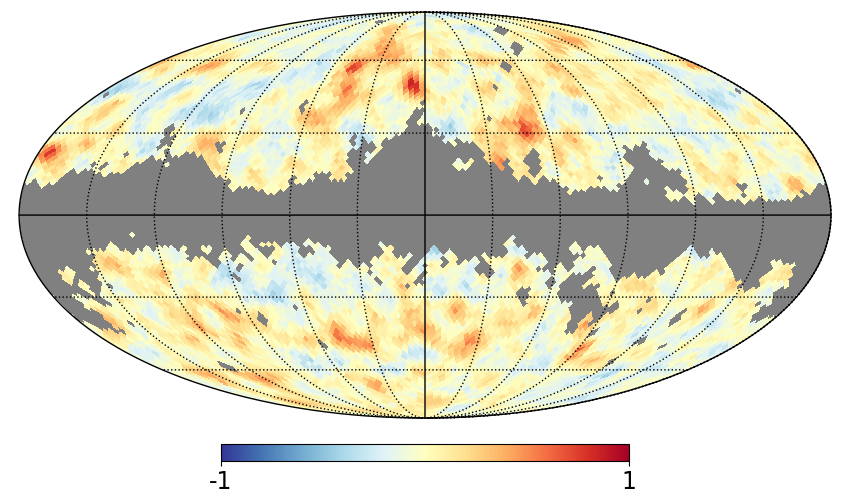
\includegraphics[width=\textwidth]{pic/band4_wmask_xsc.png}
             \caption{Band 4}
             \label{fig:contrast_map4}
        \end{subfigure}
    \caption{Mollweide projection of the 2MASS-XSC galaxy contrast maps in galactic coordinates with the combined 2MASS+WMAP mask applied ($f_{sky}=0.70$).}
    \label{fig:2MASS_maps2}
    \end{figure}
\end{frame}

\begin{frame}{Correlation Spectra Estimator}
	To estimate the correlation spectra that describe the pixelized maps $d$ with primordial signal $s$ and noise $n$ (with $\mathbf{S}$ and $\mathbf{N}$ being the corresponding covariance matrices), we could use the following likelihood function.

	\begin{align}\label{ch4:Likelihood}
	\mathcal{L}&=P(\mathbf{d}|\mathbf{C})=\frac{1}{(2\pi)^{n_\text{dim}/2}|\mathbf{C}|^{1/2}}\text{exp}\left(-\frac{1}{2}\mathbf{d}^T \mathbf{C}^{-1} \mathbf{d}\right), & \mathbf{C}&=\mathbf{S}+\mathbf{N}
	\end{align}	

	With a prior $\pi(\mathbf{S})$ we can use Bayes' Theorem to obtain
	
	\begin{equation}
	P(\mathbf{C}|\mathbf{d})\propto \pi(\mathbf{S})P(\mathbf{d}|\mathbf{C})
	\end{equation}	 
\end{frame}

\begin{frame}{Correlation Spectra Estimator}
     If we can sample from $P(\mathbf{C}|\mathbf{s},d)$ and $P(\mathbf{s}|\mathbf{C},d)$. Then we iterate

    \begin{align}
        \mathbf{s}^{i+1}&\leftarrow P(\mathbf{s}|\mathbf{C}^i,d)\\
        \mathbf{C}^{i+1}&\leftarrow P(\mathbf{C}|\mathbf{s}^{i+1},d),
    \end{align}

    to obtain a sample of $\{(\mathbf{s}^i, \mathbf{C}^i)\}$.
\end{frame}

\begin{frame}{The Blackwell-Rao Estimator}
    We can then use the Blackwell-Rao estimator to obtain an approximation for $P(C_\ell|\mathbf{d})$

    \begin{equation}
        P(C_\ell|\mathbf{d})\approx \frac{1}{N_G}\sum_{i=1}^{N_G}P(C_\ell|\sigma_\ell^i),
    \end{equation}

    where

    \begin{equation}
        \sigma_\ell^i = \frac{1}{2\ell+1}\sum_{m=-\ell}^\ell \mathbf{s}_{\ell m}\mathbf{s}_{\ell m}^\dagger.
    \end{equation}

    We then maximize the probability $P(C_\ell|\mathbf{d})$ to obtain the best-fit $C_\ell$. 
\end{frame}

\begin{frame}{Matrices Used}
	In this work, $\mathbf{s}$ and $\mathbf{S}$ are defined by
	
	\begin{equation}\label{vec_s}
	\mathbf{s}^T=(s_{00}^{tg}, s_{01}^{tg}, s_{11}^{tg}, \dots, s_{\ell_\text{max}0}^{tg}, \dots, s_{\ell_\text{max} \ell_\text{max}}^{tg}),
\end{equation}
\begin{equation}\label{matrix_S}
	\mathbf{S}=\text{diag}(S_0^{tg}, S_1^{tg}, S_1^{tg},\dots, S_{\ell_\text{max}}^{tg}, \dots, S_{\ell_\text{max}}^{tg}),
\end{equation}

where 

\begin{align}\label{s_lm=}
	\mathbf{s}_{\ell m}^{tg}&=
	\begin{pmatrix}
	a_{\ell m}^t\\
	a_{\ell m}^g
	\end{pmatrix}, &
	\mathbf{S}_\ell^{tg}&=
	\begin{pmatrix}
	C_\ell^{tt} & C_\ell^{tg}\\
	C_\ell^{tg} & C_\ell^{gg}
	\end{pmatrix}.
\end{align}

\end{frame}


\begin{frame}{Correlation Spectra Obtained}
    \begin{figure}
        \centering
        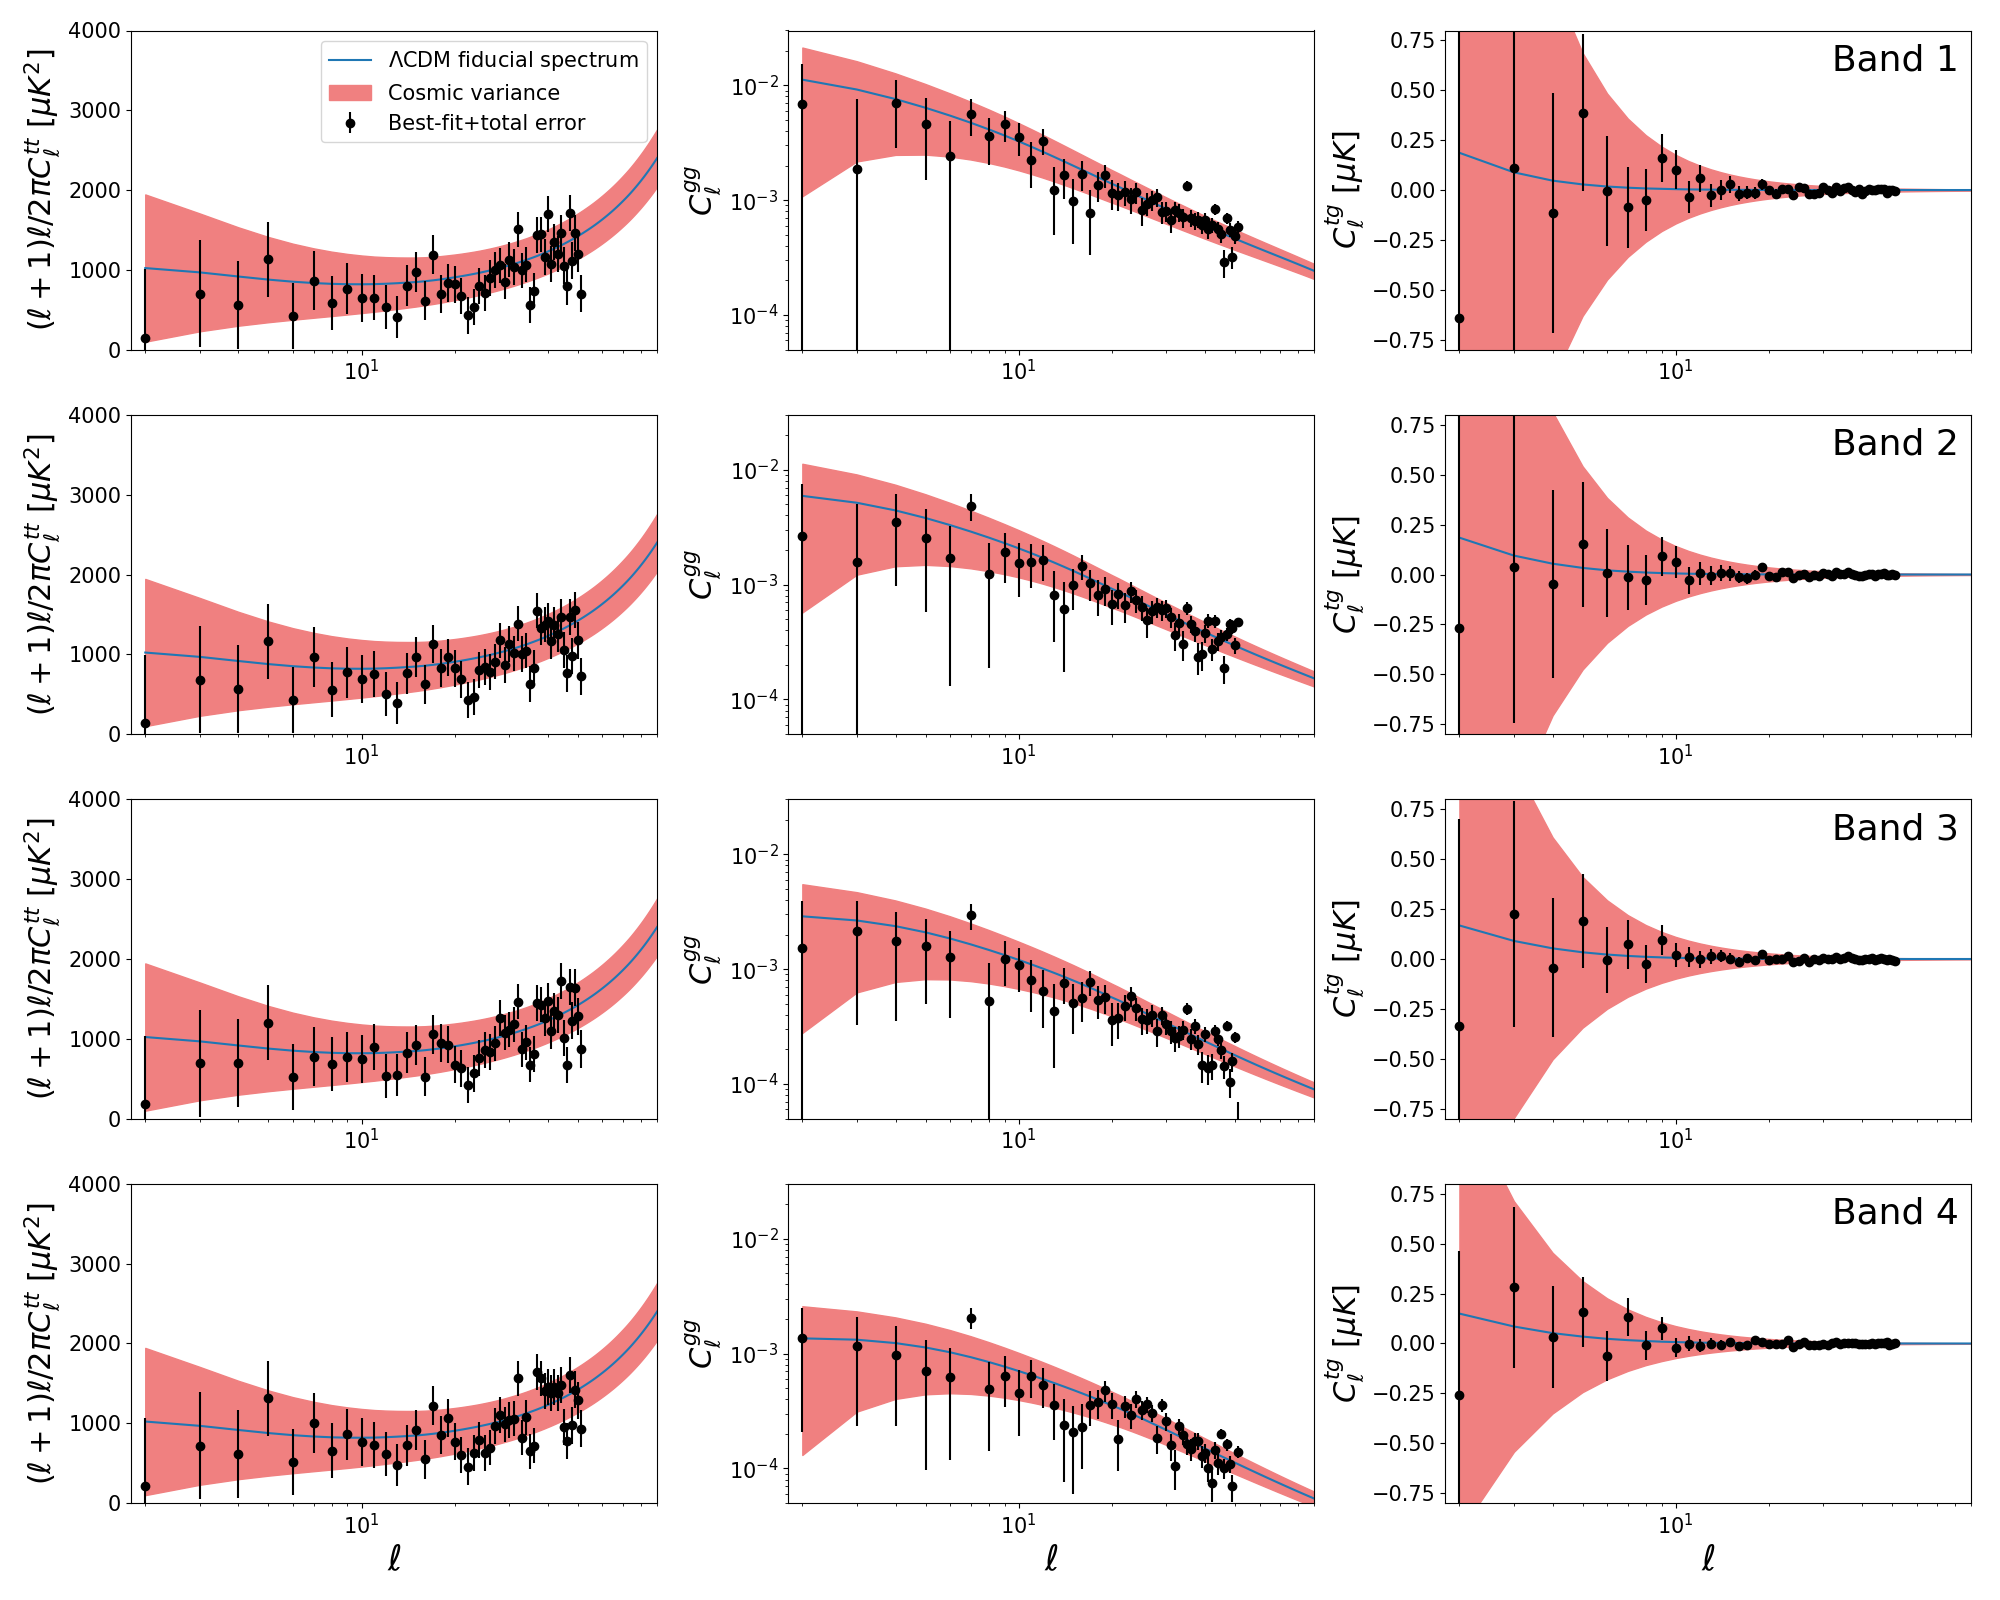
\includegraphics[width=0.7\linewidth, height=0.73\textheight]{pic/Full_Data_Plot.png}
        \caption{Comparison between theoretical correlation spectra and the ones estimated from WMAP and 2MASS.}
        \label{fig:correlations_obtained}
    \end{figure}
\end{frame}

\section{Analysis and Results}

\begin{frame}{Monte Carlo Markov Chains}
	By defining the likelihood $\mathcal{L}(C_\ell|\theta)$ and the prior $p(\theta)$, one can use Markov chains to obtain samples of each parameter in $\theta$ following the posterior
	
	\begin{equation}
		P(\theta|C_\ell)=\mathcal{L}(C_\ell|\theta)p(\theta)
	\end{equation}
	
	Joint posteriors can be easily obtained from each parameter sample, strongly simplifying data analysis for multiple parameter models.
\end{frame}

\begin{frame}{Planck Likelihoods}
	\begin{figure}
	\centering
	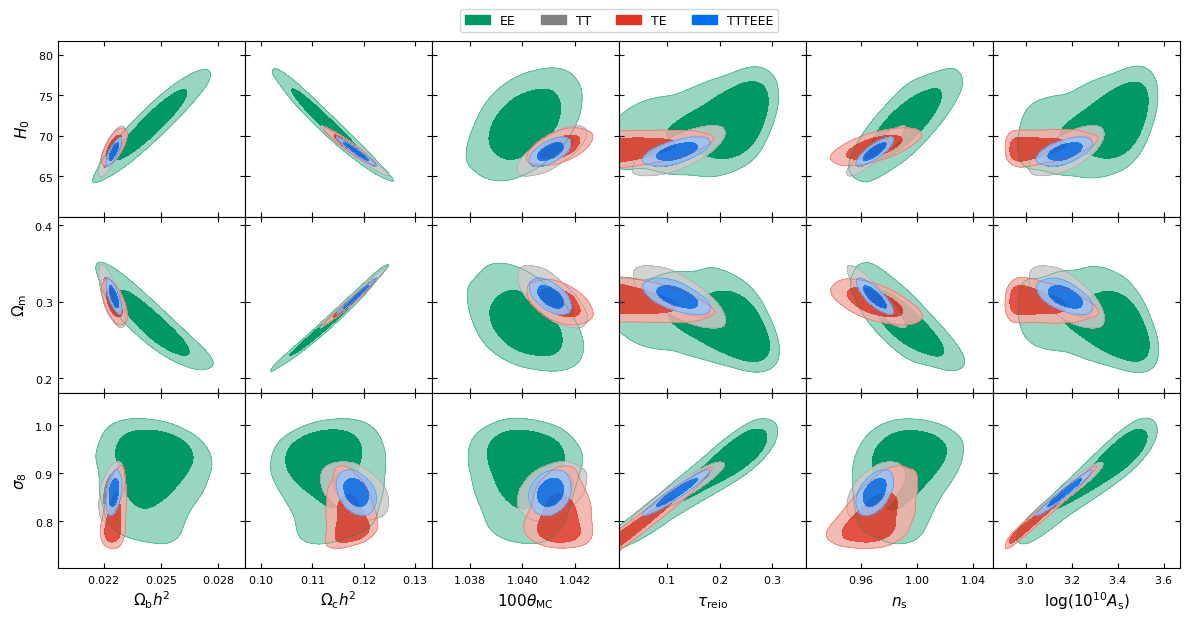
\includegraphics[width=.75\linewidth]{pic/compare_likelihoods.png}
	\caption{Joint posterior distributions of cosmological parameters using Planck’s CMB temperature (T) and polarization (E) data.}
	\label{fig:Planck_posteriors}
	\end{figure}
\end{frame}

\begin{frame}{Likelihood Profiling}
    %To analyze the data, we have opted to profile the likelihood functions applied to $\Omega_m$. 
    
    The likelihood of each point in the spectrum was assumed to be Gaussian

    \begin{equation}\label{likelihood_cl}
    	\mathcal{L}(C_{\ell\text{, theo}}^{xy}|C_{\ell\text{, data}}^{xy})=\frac{1}{\sigma_\ell \sqrt{2\pi}}\text{exp}\left[-\frac{1}{2}\left(\frac{C_{\ell\text{, data}}^{xy}-C_{\ell\text{, theo}}^{xy}}{\sigma_\ell}\right)^2\right].
    \end{equation}

    We are varying only $\Omega_m$, so $C_{\ell\text{, theo}}^{xy}$ is a functions of only $\Omega_m$. The likelihood of a full spectrum is

    \begin{equation}\label{likelihood_cxy}
    	\mathcal{L}(\Omega_m|C^{xy}_\text{data})=\prod_{\ell=2}^{\ell_\text{max}} \mathcal{L}(C_{\ell\text{, theo}}^\text{xy}|C_{\ell\text{, data}}^\text{xy}).
    \end{equation}

    The $C^{tg}+C^{gg}$ joint-likelihood is

    \begin{equation}
        \mathcal{L}(\Omega_m|C^{tg}_\text{data},C^{gg}_\text{data})=\mathcal{L}(\Omega_m|C^{tg}_\text{data})\mathcal{L}(\Omega_m|C^{gg}_\text{data}).
    \end{equation}
\end{frame}

\begin{frame}{Results for 2MASS}
    \begin{columns}
        \column{0.6\linewidth}
        \begin{figure}
            \centering
            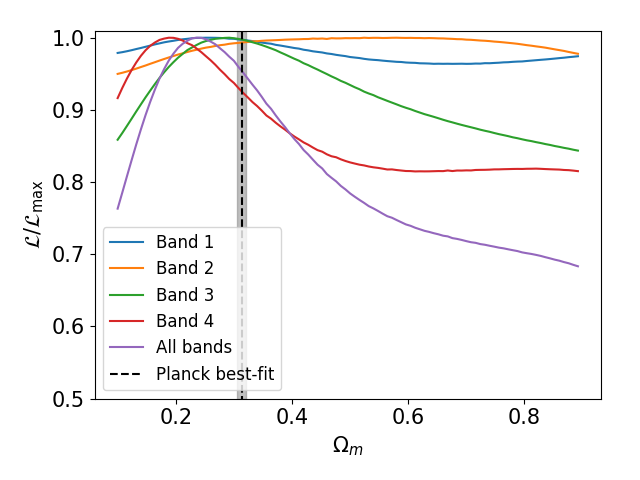
\includegraphics[width=\linewidth]{pic/profile_ctg_Nmc2e7.png}
            \caption{$C^{tg}$ only likelihood profiles.}
            \label{fig:prof_ctg}
    \end{figure}
        \column{0.4\linewidth}
        \begin{itemize}
            \item All curves are compatible with Planck;
            \item Not much constraining power on $\Omega_m$;
            \item Bands 3 and 4 -- which have the deepest selection functions -- have the most constraining power amongst all 4.
        \end{itemize}
    \end{columns}
\end{frame}

\begin{frame}{Results for 2MASS}
    \begin{columns}
        \column{0.6\linewidth}
        \begin{figure}
            \centering
            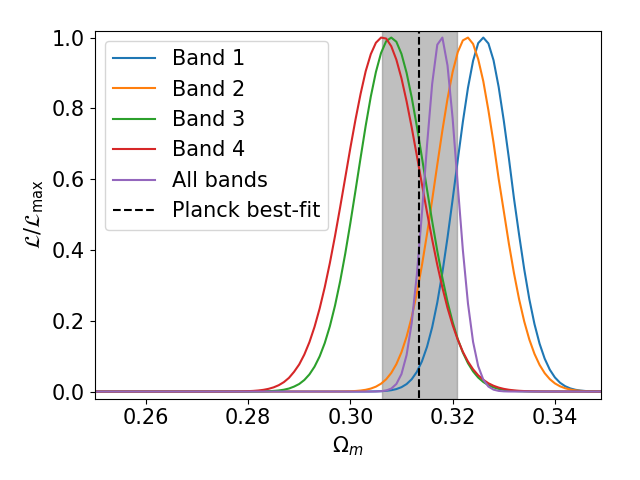
\includegraphics[width=\linewidth]{pic/profile_allbands_Nmc2e7.png}
            \caption{Joint likelihood profiles}
            \label{fig:prof_ctg_cgg}
        \end{figure}
        \column{0.4\linewidth}
        \begin{itemize}
            \item All likelihoods are compatible with Planck;
            \item Very high constraining power on $\Omega_m$ when $C^{gg}$ is introduced, comparable to Planck's;
            \item No significant difference in constraining power between each band.
        \end{itemize}
    \end{columns}
\end{frame}

\begin{frame}{Forecast for the Optimized Band}
    To estimate the behavior of a survey that follows our idealized selection function in this analysis, we have produced two synthetic cross-correlation spectra using that selection function. Both use the $\Lambda$CDM model with Planck's best-fit parameters, only differing in $\Omega_m$:

    \begin{itemize}
        \item One of the datasets was produced using Plancks best-fit of $\Omega_m=0.3153$;
        \item The other dataset was produced using $\Omega_m=0.188$, the value that maximizes the likelihood of band 4 for the $C^{tg}$ only likelihood.
    \end{itemize}

    Band 4's errors were used as estimated for both synthetic datasets.
\end{frame}

\begin{frame}{Forecast for the Optimized Band}
    \begin{columns}
        \column{0.6\linewidth}
        \begin{figure}
            \centering
            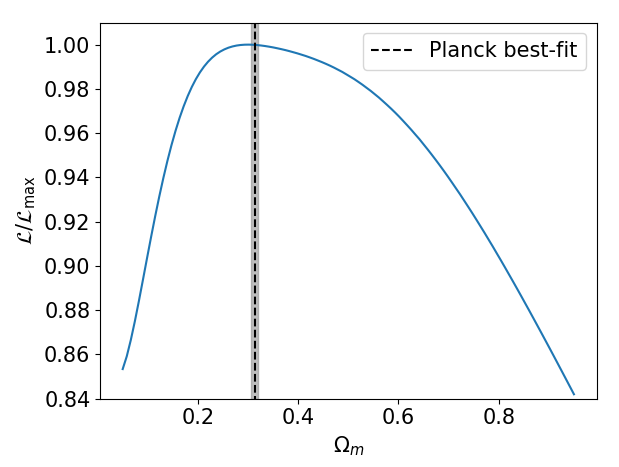
\includegraphics[width=\linewidth]{pic/profile_BestBand.png}
            \caption{Optimized band $C^{tg}$ only profile.}
            \label{fig:profile_BestBand}
        \end{figure}

        \column{0.4\linewidth}
        \begin{itemize}
            \item Constraining power still low;
            \item Reasonable improvement in the constraining power.
        \end{itemize}
    \end{columns}
\end{frame}

\begin{frame}{Discussion}
    \begin{itemize}
        \item The optimized band being deeper than 2MASS means errors on the spectra should be lower, meaning the errors used are overestimated, which indicates the constraints could be better for a real survey following our optimized selection function;
        \item The optimized band was not found by optimizing the $\Omega_m$ constraints, but rejecting the null cross-correlation hypothesis. $\Omega_m=1$ leads to $C_\ell^{tg}=0$, and the fast decrease in likelihood for higher $\Omega_m$ is noticeable.
    \end{itemize}
\end{frame}

\section{Conclusions}

\begin{frame}{Conclusions}
    \begin{itemize}
        \item We have obtained the likelihood profiles for $\Omega_m$ obtained from cross-correlation data by studying the ISW effect;
        \item The constraints obtained using only $C^{tg}$ were not strong, but can be used as a complement to other datasets for a combined analysis;
        \item In the 2MASS catalog, the 2 deepest bands -- bands 3 and 4 -- yielded better constraining power;
        \item The Planck collaboration also studied the ISW effect using the cross-correlation spectrum\cite{cross_corr:Planck}, obtaining significantly better results with deeper surveys (SDSS\cite{NVSS} and Planck's Kappa map).
    \end{itemize}
\end{frame}
\begin{frame}{Conclusions}
    \begin{itemize}
        \item An optimized band capable of maximizing the ISW signal was obtained, prioritizing galaxies at higher redshifts and increasing the cross-correlation signal in a region less affected by cosmic variance;
        \item The likelihoods obtained for artificial data calculated using the optimized band improved the constraints on $\Omega_m$;
        \item Combining different matter tracers leads to improved results overall.
    \end{itemize}
\end{frame}

\begin{frame}
    \begin{center}
        {\Huge\calligra Thank You}
    \end{center}
\end{frame}

\section*{Extras}

\begin{frame}{Extra Content}
    Discussão de Future prospects
\end{frame}

\begin{frame}{Extra Content}
	More extras
\end{frame}

\begin{frame}[allowframebreaks]{Bibliography}
\printbibliography
\end{frame}

\end{document}